% \subsubsection{Image Change Detection Algorithm}
% \subsubsection{Throw Detection Algorithm}
\subsubsection{Employed Algorithm}
\label{subsubsec:algorithm}
% \todo[inline]{No citations?! Or OpenCV?! Or Baumer?!}

% image change detection algorithm vs throw detection / throw detection mechanism / throw detection algorithm => throw detection employs icda

% Goal of the throw detection is to extract the valid frames of a throw from the continous data stream
  % valid frames have object on them, invalid frames are empty (background)
% real-time
% serial process, 200 fps => >5 ms to process each frame
% not a lot of time for a complex (fancy) algorithm => simplest one possible is used
  % for the throw detection algorithm a simple image change detection algorithm is used

% Algo: computation of the difference and comparison to a threshold to detect changes in the picture

% what this sections does with the listings

% Due to the in section {} mentioned bandwidth limitations of the U3V interface the raw bayer is processed
  % conversion to BGR8 takes too long! => use raw bayer for the detection
% Saving images takes time + unnecessary => saving at the end!
  % see section \ref

% buffers

% frame_id (FID) to keep track of ...
% uses 2 flags and 2 "pointers" to the buffer

% compared against threshold (if mean_diff < threshold, considered to be no change [equal sign])

% throw begin and throw end, what happens

% Why are the last two frames are not valid?
  % only possible to detect the end when there is no change any longer

The goal of the throw detection is to extract valid frames of a throw --- with objects on them --- from the continous data stream of the camera.
Therefore, the throw detection needs to work in real time.
At a frame rate of \SI{200}{fps}, there is $<\SI{5}{ms}$ to process a single frame (without the use of parallel computing).
Due to this time constraint, a simple image change detection algorithm is employed.

\paragraph{Image Change Detection Algorithm}
\vspace{-20pt}
\begin{enumerate}
  \item Compute the absolute difference between the current and the last frame
  \item Compute the average among all the pixels of the difference
  \item Compare the mean difference against a threshold value
\end{enumerate}

This section describes only selected parts of the implementation.
The complete listing of the throw detection can be found in appendix \ref{app:throw_detection}.
The implementation of the difference computation and the average among all the pixels is described in section \ref{subsubsec:difference_computation}.
Furthermore, the way the threshold value is obtained is documented in section \ref{subsubsec:threshold}.

Due to the bandwidth limitations of the U3V interface mentioned in section \ref{subsubsec:usb3_vision_interface}, the received images are in the raw Bayer pixel format.
A conversion from the Baumer \texttt{BayerRG8} to \texttt{BGR8} takes too long an therefore the raw frames are processed.
Moreover, the valid images are only saved on the hard disk at the end of a throw, as this also takes a lot of time (see section \ref{subsubsec:saving_images}).

For the above reasons, two image buffers are used.
The received images are stored in Baumer \texttt{BGAPI2::Buffer} objects (see section \ref{subsubsec:baumer_buffer}).
To save the images later on, a circular buffer for OpenCV matrices (\texttt{cv::Mat}) is used.
This is documented in section \ref{subsubsec:opencv_buffer}.
The size of those image buffers (\texttt{BS}) determines the max. amount of valid frames $N_\text{max}$ that can be captured.

To keep track of the present and past frames, a frame id (\texttt{FID}) is utilized.
Furthermore, two flags are used to mark the beginning and the end of a throw.

Whenever the mean difference between two consecutive frames is greater than or equal to the threshold, they are considered to be different ($\ne$).
Otherwise, the two frames are considered to be equal ($=$).

Once two consecutive frames are different, the flag \texttt{throw\_bgn} is set to \texttt{true} and the current \texttt{FID} is saved in \texttt{throw\_bgn\_idx}.
The current and all subsequent frames --- except for the last two --- belong to the detected throw until two consecutive frames are no longer different.
In this case, the flag \texttt{throw\_end} is set to \texttt{true} and the current \texttt{FID} is saved in \texttt{throw\_end\_idx}.

The last two frames are not valid due to the way the throw detection works.
The first invalid frame occurs when the object leaves the image, as this is still a change in the image and thus not detected.
The second invalid frame results from the fact that the following images are only now the same and therefore the current \texttt{FID} is saved.

Figure \ref{subfig:algorithm_general_case} shows the general case of the just described throw detection.
As already mentioned, the max. amount of valid frames $N_\text{max}$ depends on the image buffer size (\texttt{BS}).
To properly detected a throw, the amount of valid frames $N$ must meet the condition
\[
  N \in \{1..(\text{BS}-2)\}.
\]
In the current implementation, an image buffer size of \SI{1000}{} is used and therefore $N_\text{max} = \SI{998}{frames}$.
An example of three valid frames ($N = 3$) is shown in figure \ref{subfig:algorithm_example_3}.

\begin{figure}[H]
  \centering
  \begin{subfigure}[b]{\textwidth}
    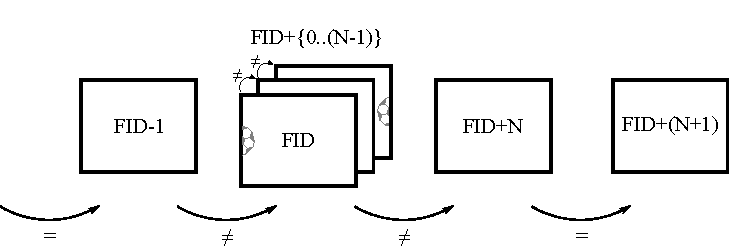
\includegraphics[scale=0.85]{algorithm}
    \caption{General case with $N \in \{1..(\text{BS}-2)\}$}
    \label{subfig:algorithm_general_case}
  \end{subfigure}
  \begin{subfigure}[b]{\textwidth}
    
\includegraphics[scale=0.85]{algorithm_ex_1}
    \caption{Example of $N_\text{min} = 1$}
    \label{subfig:algorithm_example_1}
  \end{subfigure}
  \begin{subfigure}[b]{\textwidth}
    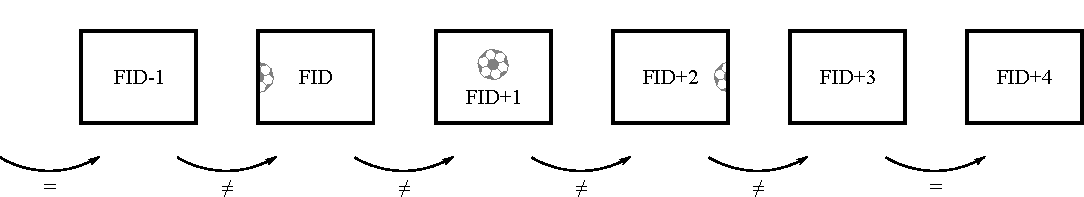
\includegraphics[scale=0.85]{algorithm_ex_3}
    \caption{Example of three valid frames ($N = 3$)}
    \label{subfig:algorithm_example_3}
  \end{subfigure}
  \caption{Illustration of the throw detection}
  \label{fig:throw_detection}
\end{figure}

Listing \ref{lst:throw_detection} shows the implementaion of the throw detection.
Due to the specific implementation, it is possible to detect a single frame change.
This means that the image changes between two consecutive frames and then stays the way it is (e.g. sudden change of the ambient light).
Such a glitch is not a valid throw and shall therefore be ignored (see line \ref{lst:ln:glitch_removal}).
Figure \ref{subfig:algorithm_example_1} shows that a valid throw of an object would create at least two changes between individual frames.
The first one by entering and the second one by leaving the frame.

\begin{lstlisting}[style=C++, caption={Throw detection and glitch removal}, label=lst:throw_detection]
  if (mean_diff >= threshold) {
      if (!throw_bgn) {
        throw_bgn_idx = frame_id;
        throw_bgn = true;
      }
  } else {
    if (throw_bgn) {
      throw_end_idx = frame_id;

      // Remove glitches (single frame changes)
      if ((throw_end_idx - throw_bgn_idx) == 1) {(*\label{lst:ln:glitch_removal}*)
        throw_bgn = false;
      } else {
        throw_end = true;
      }
    }
  }
\end{lstlisting}

As long as no throw is detected, the current Baumer \texttt{Buffer} object is released after each processed frame (see listing \ref{lst:buffer_release}).
Whenever a glitch is removed, the size of the Baumer image buffer (\texttt{BS}) is reduced by one.
This is due to the fact that no reference to past \texttt{Buffer} objects is kept.
Such a reference is necessary to release the respective buffer entry.
It would be easy to solve this by keeping track of at least one past \texttt{Buffer} object.
However, this is not necessary, provided that the buffer size is large enough.

% BUG: Should not be released directly but with a delay of one!
\begin{lstlisting}[style=C++, caption={Release of the filled Baumer \texttt{Buffer} object}, label=lst:buffer_release]
  if (!throw_bgn) {
    pBufferFilled->QueueBuffer();
  }
\end{lstlisting}
